\chapter{Bounded principle curvatures}

Note that there sets in $\RR^3$ bounded by a closed surface $\Sigma$ with principle curvatures at most 1 by absolute value
that do not contain a ball of radius 1.

\begin{wrapfigure}{r}{33 mm}
\vskip-4mm
\centering
\includegraphics{mppics/pic-34}
\vskip0mm
\end{wrapfigure}

For example the region between two spheres with large close to each other radiuses. 
This region can be made arbitrary thin and the curvature of the boundary can be made arbitrary close to zero.

The same example works in the plane --- a pair of circles with arbitrary small curvature can bound arbitrary thin region.

\begin{thm}{Advanced exercise}
Suppose a set $V\subset \RR^3$ is bounded by a closed surface $\Sigma$ with principle curvatures at most 1 by absolute value.
Assume that $V$ does not contain a ball of radius $\tfrac1{100}$.
Show that $\Sigma$ has two components of the same topological type; 
that is, both can be written in a parametric form with the same parameter domain. 
\end{thm}


The same example would work for the curves if we allow boundary of the plane figure to be not connected.
The following question might look like a right 3-dimensional analog of the moon in a puddle problem (\ref{thm:moon}).

\section{Lagunov's example}

\begin{thm}{Question}
Assume a set $V\subset \RR^3$ is bounded by a closed connected surface $\Sigma$ of bounded curvature.
Is it true that $V$ contains a ball of radius 1?
\end{thm}

It turns out that the answer is still ``no'', the following example was constructed by Vladimir Lagunov \cite{lagunov}.


\parit{Construction.}
Let us start with a body of revolution $V_1$ with the cross section shown on the diagram.
The boundary curve of the cross section is made by 6 vertical line segments that smoothly jointed into 3 closed simple curves. 
The boundary of $V_1$ has 3 components, each of which is a sphere.

\begin{figure}[h!]%{r}{43 mm}
%\vskip-4mm
\centering
\includegraphics{mppics/pic-33}
\vskip0mm
\end{figure}

A simple computation shows that if the curvature of all curves is at most 1 then the boundary surface of $V_1$ has priniple curvatures at most 1 by absolute value.

At most of the places $V_1$ can be made arbitrary thin,
the only thick place is where all tree spheres come together;
it could be arranged that the radius of the maximal ball just a bit above 
\[r_2=\tfrac2{\sqrt{3}}-1< \tfrac16.\]
This the radius of the smaller circle tangent to three unit circles that tangent to each other.


It remains to modify $V_1$ to make its boundary connected without  getting larger balls inside.

Note that each sphere in the boundary contains two flat discs;
they come into pairs close lying to each other. 
Let us drill thru two of such pairs and reconnect the holes by an other body of revolution which axis is shifted but stays parallel to the axis of $V_1$.
Denote the obtained body by $V_2$; its cross section of the obtained body is shown on the diagram. 

Then repeat the operation for the other two pairs.
Denote the obtained body by $V_3$; its cross section of the obtained body is shown on the diagram.

It is easy to see that the boundary of $V_3$ is connected
and assuming that the holes are large its boundary can be made so that its principle curvatures is still at most $1$.
\qeds

\begin{thm}{Claim}
The surface of $V_3$ has genus 2.
\end{thm}


\parit{Proof.}
Note that the boundary of $V_1$ is three spheres.

When we drill a hole, we make one hole in two spheres and two holes in one shpere.
We reconnect two spheres by a tube and obtan one sphere
and connect two holes of one sphere by a tube we get a torus.

At the second operation we make a torus from the remaining sphere and connect it to the other torus by tube.
This way we get a sphere with two handles; that is, it has genus 2.
\qeds

\begin{thm}{Exercise}
Assume $V$ is a body of revolution in $\RR^3$ and its boundary is a connected surface with principle curvatures at most 1 by absolute value.
Show that $V$ contains a unit ball.
\end{thm}

\begin{thm}{Exercise}
Assume $V$ is a convex body in $\RR^3$ bounded by a surface with principle curvatures at most 1.
Show that $V$ contains a unit ball.%
\footnote{Hint: Consider a maximal ball in $V$ and apply Exercise~\ref{ex:projection} for a right choice of projection.}
\end{thm}





\begin{thm}{Exercise}
Modify Lagunov's construction so that the boundary surface would be a sphere with 4 handles.%
\footnote{Hint: Combine two examples together using the same construction (or use the spherical annulus together with Lagunov's example).}
\end{thm}



\begin{thm}{Advanced exercise}
Show that the bound in the Lagunov's example is optimal.
That is, if a body $V\subset \RR^3$ is bounded by a connected surface  $\Sigma$ with principle curvatures at most 1, then $V$ contains a ball of radius $r_2$.
\end{thm}

\section{On embedded sphere}


\begin{thm}{Advanced exercise}
Note that the body $V$ in the example of Lagunov is constructed by thikening a surface that has a singular curve at surface meets at angles $120\degree$.
Show that this way one can not obtain a body bounded by a sphere.
\end{thm}

In fact one can show that if a body $V\subset \RR^3$ is bounded by a sphere $\Sigma$ with principle curvatures at most 1, then $V$ contains a ball of radius $r_3=\sqrt{\tfrac32}-1>\tfrac15$,
which is the radius of smaller sphere that tangent to three unit sphere that are tangent to each other.
Moreover this bound is optimal.

An example of such body can be obtained by thickening the so called Bing's house.
It is certain surface which singularities are formed by three curves that meet at two points;
four ends at each point.
The remaining surface of Bing's is smooth and has bounded principle curvatures;
we can assume that they are bounded by arbitrary small value.

At the singular curves curves theree pieces of surface have to come at angles $\tfrac23\cdot\pi$ and at the sigular points 6 pieces of surface should come together forming 6 tringles with vertex in the center of regular tetrahedron and the bases at its 6 edges.
Thickening of sufficiently large Bing's house of that type produces the optimal bound $r_3$ on the maximal ball that it contains.

\begin{wrapfigure}{o}{52 mm}
\vskip-0mm
\centering
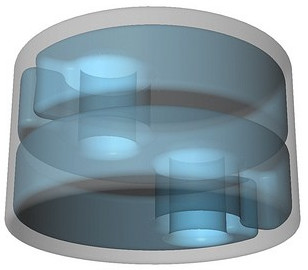
\includegraphics[scale=.45]{pics/thickened-bing's-house}
\vskip-0mm
\end{wrapfigure}

The thickening of Bing's house shown on the picture can not give the optimal bound,
but still it can produce an example of embedded sphere that does not surround a ball of radius 1.

This picture is very similar to the Lagunov's example described above --- it can be obtained by filling the rings in the section of $V_3$ by a thickened discs. 

This picture of a taken from posts of Ken Baker \cite{baker};
this post has many other beautiful pictures that help to visualize Bing's house.

